\documentclass[11pt, twoside, reqno]{article}
\usepackage{amssymb, amsthm, amsmath, amsfonts}
\usepackage{graphicx}
\usepackage{color}
\usepackage{hyperref}
\usepackage{verbatim}
\usepackage[toc,page]{appendix}
\usepackage{listings}
\usepackage{float}
\usepackage[shortlabels]{enumitem}
\setlist[enumerate, 1]{1\textsuperscript{o}}

\definecolor{codegreen}{rgb}{0,0.6,0}
\definecolor{codegray}{rgb}{0.5,0.5,0.5}
\definecolor{codepurple}{rgb}{0.58,0,0.82}
\definecolor{backcolour}{rgb}{0.95,0.95,0.92}

\lstdefinestyle{mystyle}{
    backgroundcolor=\color{backcolour},
    commentstyle=\color{codegreen},
    keywordstyle=\color{magenta},
    numberstyle=\tiny\color{codegray},
    stringstyle=\color{codepurple},
    basicstyle=\footnotesize,
    breakatwhitespace=false,
    breaklines=true,
    captionpos=b,
    keepspaces=true,
    numbers=left,
    numbersep=5pt,
    showspaces=false,
    showstringspaces=false,
    showtabs=false,
    tabsize=2
}

\lstset{style=mystyle}

\begin{document}

\label{label}
\section{Introduction}
\hspace{0.2in} Mathematical models like the one we intend to build run on large amounts of data. Just under three million tweets were collected for this experiment. Obviously that number is too large to be done manually. A script automated a pipeline that collected tweets matching keywords and saved them to be analyzed. 

\begin{figure}[H]
	\centering
	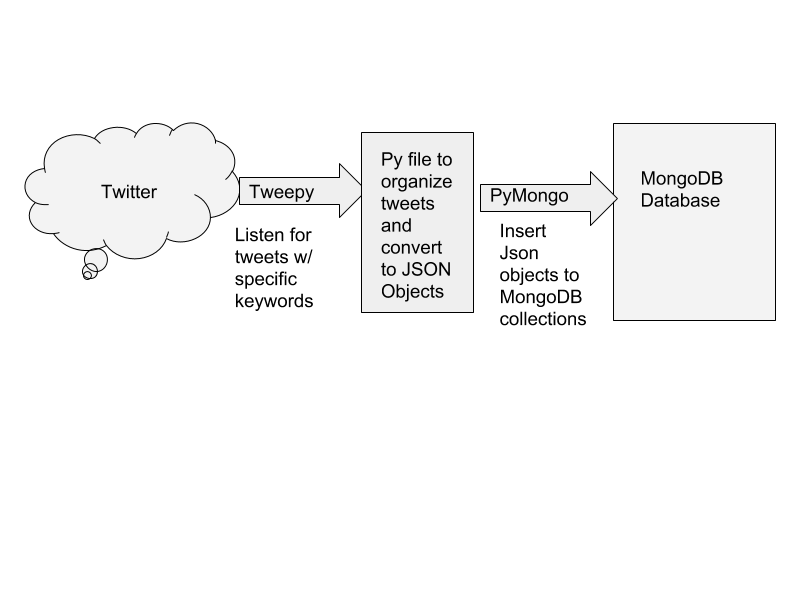
\includegraphics[scale=0.5]{data_collection}
	\caption{A high level overview of the tweet collection pipeline}
	\label{fig:datacollection}
\end{figure}

The cloud in Figure \ref{fig:datacollection} represents all of the tweets on Twitter at any given moment. The arrow represents the streamer. The streamer is a data structure that will monitor Twitter and download all tweets that match certain keywords. Those tweets that the streamer pulls need to be stored. To do that they need to be formatted into JSON or JavaScript Object Notation. When they are, they will be inserted into a database using the management software MongoDB. 

To complete all those actions in python, we'll need to use Application Package Interface (API). APIs are how scripts and other pieces of code can interact with software such as Twitter or MongoDB. Tweepy is the Twitter API and Pymongo is the Python API. 
 
To summarize, the pipeline process can be distilled into three separate tasks. 
\begin{enumerate}
	\item Building a tweet streamer to ``listen'' to tweets based on keywords
	\item Preprocessing the tweets into JSON notation
	\item Storing processed tweets into a database running MongoDB 
\end{enumerate}
The python script that does this can be found in Appendix B. The explicit instructions on operating the script can be found in Appendix A. 


\section{Streaming Tweets}
\label{sec:streaming}
\hspace{0.2in} There are two ways to gather tweets using the Python Twitter API. One is to query a profile or a search term. This method is not preferred for several reasons. First, Twitter has put a hard cap on the number of tweets each query can return at one time. To query every single tweet about a subject will need repeated queries of the maximum amount. Considering that the actual number of tweets is unknown, this is a time-consuming loop that has no estimate-able end. Next, Twitter's search function naturally promotes tweets that have more engagement (likes, comments, and retweets). Collecting only those tweets means we put together an incomplete and biased data set. 

The other way to gather tweets is to stream tweets. A Tweepy stream monitors live twitter content and returns all tweets that contain a given set of keywords while the stream is active. Streaming has the disadvantage of gathering only live tweets - it does not search tweets from before it started running. , streaming has the advantage of gathering all tweets that meet the keyword requirement irrelevant of engagement level. 

Tweepy's Streamer is an abstracted object. That means that it provides the outline for how a streamer should work, but the specifics are left up to the user. The streamer has functions or methods that need to defined so that the streamer understands what to do with the tweets it gathers. 

The methods that need to be defined here are on\_connect, on\_error, and on\_data. The first two are simple. On\_connect is used to connect to the internet, and it confirms when the stream is live. If the stream crashes - which can happen for several reasons - on\_error informs the user why the stream stopped. This can happen for many reasons which include: exceeding the rate limit (tweets streamed per second), a faulty internet connection, and more. 

The last method on\_data is where the streamed tweets are received and processed.  Streamed tweets are returned by a streamer in a python dictionary format with the keys as attributes (user, text, etc.). As mentioned earlier, MongoDB only takes in objects in JSON format. The dictionaries need to be converted - which is what happens in the preprocessing.  This is a process that happens simultaneously so that there is no need to intermediately store the tweets before they're ready to be stored in the database. 

\section{Databases}
\hspace{0.2in} The on\_data method from section \ref{sec:streaming} is inserting tweets into a database. In this section, we'll explore what databases are and how they're specifically applied in this project.
\subsection{Overview}
The term database refers to any structure that electronically stores data. In extension, the Database Management System is the program that allows users to interact with the database. In this paper, when the term database is used, it refers to both the structure and the system. 

There are several types of databases. These types are classified by the way the data is organized inside the structure. The relational database model uses tables with rows and columns to store information. Relational databases use Structured Query Language or SQL to organize, extract, and insert data. This has become the industry default which leads us to refer to non-relational databases colloquially to as "NoSQL". Non-relational use an object-oriented approach with different query languages. Each individual entry is an object all by itself and searches are done through a tagging system. 

Databases offer several advantages that other storage options like Excel or CSVs will not. For one, data integrity is higher. An example of better integrity is that one field can't have entries of different types across all objects. In Excel, a user field could have both a string or an integer and the program would except it without fault. In a database, the error would be spotted and left to be changed at the user's discretion.

Another advantage is the ability to scale a database. They are built to handle gigabytes and even terabytes of data. Excel by contrast is limited to around one million rows. The ability to quickly search and sort through millions of tweets as well as the flexibility to manipulate said data is something that isn't available to Excel.

The question that remains is which database to use here? The database will have to deal with millions of tweets, be able to search terms quickly, and handle inconsistencies in object size. Some tweets after all have more information than others (location, images, etc.) It's been mentioned several times earlier in this chapter, but a non-relational database running MongoDB was chosen. The next section will give an overview of what MongoDB is and how it's the best choice for this project. 

\subsection{MongoDB}
\hspace{0.2in} MongoDB is a popular open source non-relational database management system. It has an efficient query language as well as a well-defined API Pymongo. In a MongoDB database, each tweet is an object in JSON format. These objects are stored in collections and the collections are stored in a database:

\begin{figure}[H]
	\centering
	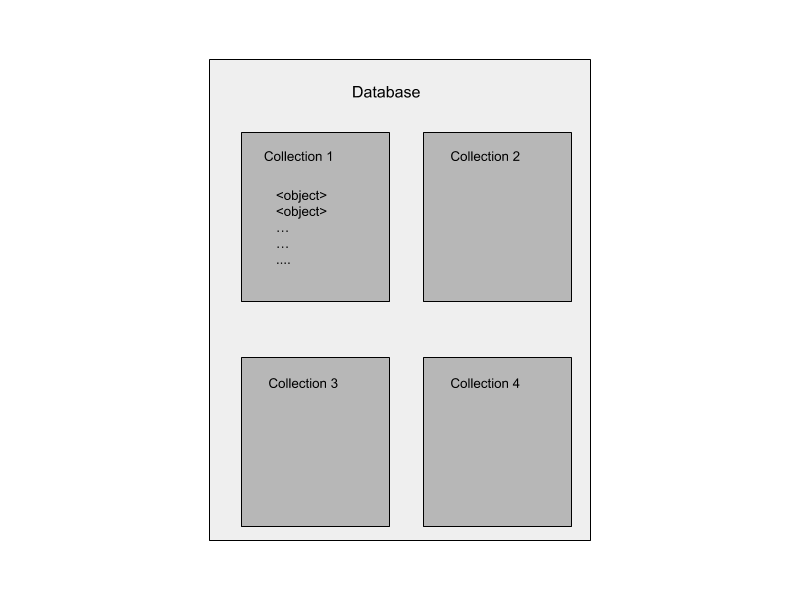
\includegraphics[scale=0.5]{database}
	\caption{MongoDB's storage organization. Tweets are stored individually in collections which are stored overall in a database.}
	\label{fig:dbstructure}
\end{figure}

These JSON objects have fields, populated with values. MongoDB allows a user to query collections using field title as well as field values. The queries can be exact matches, relational operators for integers, etc. For example, you can query tweets by date, or location (by exact match) or query all tweets that have more than a hundred retweets(relational). You can also query sub-matches. That means conditions within a field and not an exact match. Sub-matches might be searching for all tweets that contain the words ``Donald Trump'' or all tweets for all day rather than an exact time down to the second. 

MongoDB has a mongo shell through which a user can interact with the databases. This is a convenient way to access quick information about a database. Information on using the mongo shell is in Appendix A. For longer and larger actions, we use the Python API Pymongo to write python scripts. Pymongo allows us to insert, edit, and query databases and manipulate the output. 

For more specifics on Pymongo and setting up MongoDB, refer to Appendix A or the Pymongo documentation.

\section{Data Collection}
\hspace{0.2in} 
The first step of implementing the pipeline outlined at the start of the chapter is building the streamer. The first step of streaming requires search terms to stream. The search terms were taken from house and senate races, as well as general terms that refer to the 2018 midterms. Search terms for Senate and House Races were tweets about the candidates as well as a hashtag referring to the race. 

To direct the tweets streamed into a database, the on\_data method is defined. This method is designed for the streamer to deal with the tweets it selects.

\begin{verbatim}
def on_data(self, data):
	try:
            client = MongoClient(MONGO_HOST)

            # Use twitterdb database. If it doesn't exist, it will be created.
            db = client.miscdb

            # Decode the JSON from Twitter
            datajson = json.loads(data)

            #grab the 'created_at' data from the Tweet to use for display
            created_at = datajson['created_at']

            #print out a message to the screen that we have collected a tweet
            print("Tweet collected at " + str(created_at) + " " + datajson['text'])

            #insert the data into the mongoDB into a collection called twitter_search
            #if twitter_search doesn't exist, it will be created.
            db.misc.insert(datajson)
        except Exception as e:
           print(e)
\end{verbatim}

The tweet is converted into a JSON object and inserted into a database and collection of the users choice. This is a barebones definition. Sorting, editing, and adding information to tweets would all be defined here. 

The timing of the election in November of 2018 was a hard deadline for streaming tweets. Streaming tweets was a higher priority than having them sorted into neat collections regarding races. Therefore, all the tweets were shoved into one collection without being sorted. This meant that the sorting process was delayed until data exploration and model building. 

The data collection process ran through three separate scripts, each with a different set of search terms. Those three scripts fed into three different collections in one over-arching database. Together they assemble a diverse dataset that contains just under three million tweets. Chapter 4 explores the assembled data set.  

\end{document}

